% Sample Paper for Poster Conference
%( without guarantee:-)) 
%send your comment to xrund@fel.cvut.cz
%
\documentclass{poster16}
% 
%----------------------------------------------------------
%             THIS IS THE PLACE FOR YOUR FAVORITE PACKAGES
%
%\usepackage[latin2]{inputenc}%
%\usepackage{babel}% 
%\usepackage{czech}%
%\usepackage{psfrag}
%\usepackage{amsmath}
%\usepackage{pifont,amssymb}

\begin{document}
%----------------------------------------------------------

%----------------------------------------------------------
%               THIS IS THE PLACE OF THE TITLE
%
\title{3D printed rocket - platform for student experiments}
%----------------------------------------------------------
%               THIS IS THE PLACE FOR THE AUTHORS NAMES AND THE TITLE FOR HEADINGS
%
\headtitle{F. S. AUTHOR, S. S. AUTHOR, SAMPLE PAPER FOR POSTER 2016 CONFERENCE}
%----------------------------------------------------------
%               THIS IS THE PLACE FOR THE AUTHORS NAMES - ALL AUTHORS MUST HAVE A STUDENT STATUS!!!

%
\author{Jakub Kakona \affiliationmark{1}}
%----------------------------------------------------------
%              THIS IS THE PLACE FOR AFFILIATIONS
%
\affiliation{%
\affiliationmark{1}Dept. of Radio engineering, Czech Technical University, Technick\'a 2, 166 27 Praha, Czech Republic}
  \email{kakonjak@fel.cvut.cz}
%--------------------------------------------------------------


\maketitle

%----------------------------------------------------------
%               THIS IS THE PLACE FOR ABSTRACT

\begin{abstract}
The rocket sounding is a well known atmospheric research tool. In addition to the science and technology, sounding rockets also provide invaluable tools for education and training. Sounding rocket mission at a university provides an excellent research opportunity, in which the students carry out the project through all of its stages  --  from conception to hardware design to flight to data analysis and, finally to the publication of the results.  This "hands on" approach provides the student with invaluable experience of understanding the space flight mission as a whole.
\end{abstract}

%----------------------------------------------------------
%               THIS IS THE PLACE FOR KEYWORDS
\begin{keywords}
Rocket experiments, 3D printing, sounding rocket, experimental platform, scientific instrumentation.
\end{keywords}

%----------------------------------------------------------
%               HERE WRITE YOUR PAPER

\section{Introduction}

Scientific rocket experiments were relatively common in atmospheric research over the past decades \cite{rocket_sounding}. Although the rocket sounding is similar to the use of hight-altitude balloons, the rocket can reach a high altitude very quickly in a well defined time window and with relatively precise coordinates. Furthermore, the rocket lunch itself can be passed under an  unfriendly weather conditions. Therefore this type of sounding has several benefits over balloon sounding. It can be used for precise in situ measurement of interesting atmospheric events. Such events could be tornado measurements, storm measurements and other usually localised but very interesting and probably dangerous processes which need an automated measuring systems. 

Unfortunately, the rocket sounding is quite inaccessible for widespread use, specifically when used as a part of measurement networks. One of main reasons of that is the price of the rocket lunch vehicle, caused mainly by the one-off use of a relatively expensively machined device. 
Because of that a different manufacturing and design process is needed for rocket construction. 
For appropriate range of rocket vehicles the state of the art but inexpensive FDM 3D printig process could be used. A specially designed rocket body is needed when using an additive manufacturing process instead of classical machining. 

\section{Design evolution}

We decided to use the Fused deposition modelling (FDM) additive manufacturing technology as a best candidate for small and medium sized sounding rocket vehicle. The main reason for that decision was a fact, that this type of 3D printing technology is widely accessible and is of sufficient quality to build rocket body which could withstand the mechanical and aero-dynamical stresses during the rocket lunch. The second reason is the fact that this type of technology is relatively  cheap in comparison to other additive manufacturing methods. 
But there also exist technological limits due to the fact that not all shapes could be 3Dprinted. The problematic geometry include overhanging surfaces or large number of very small details in printed volume. 
The design of rocket vehicle therefore must have special construction which allows reliable printing without costly model specific G-code tweaking. Which is common practice to print poorly designed model on unsuitable printer. 

\begin{figure}[ht]
\begin{center}
\resizebox{\linewidth}{!}{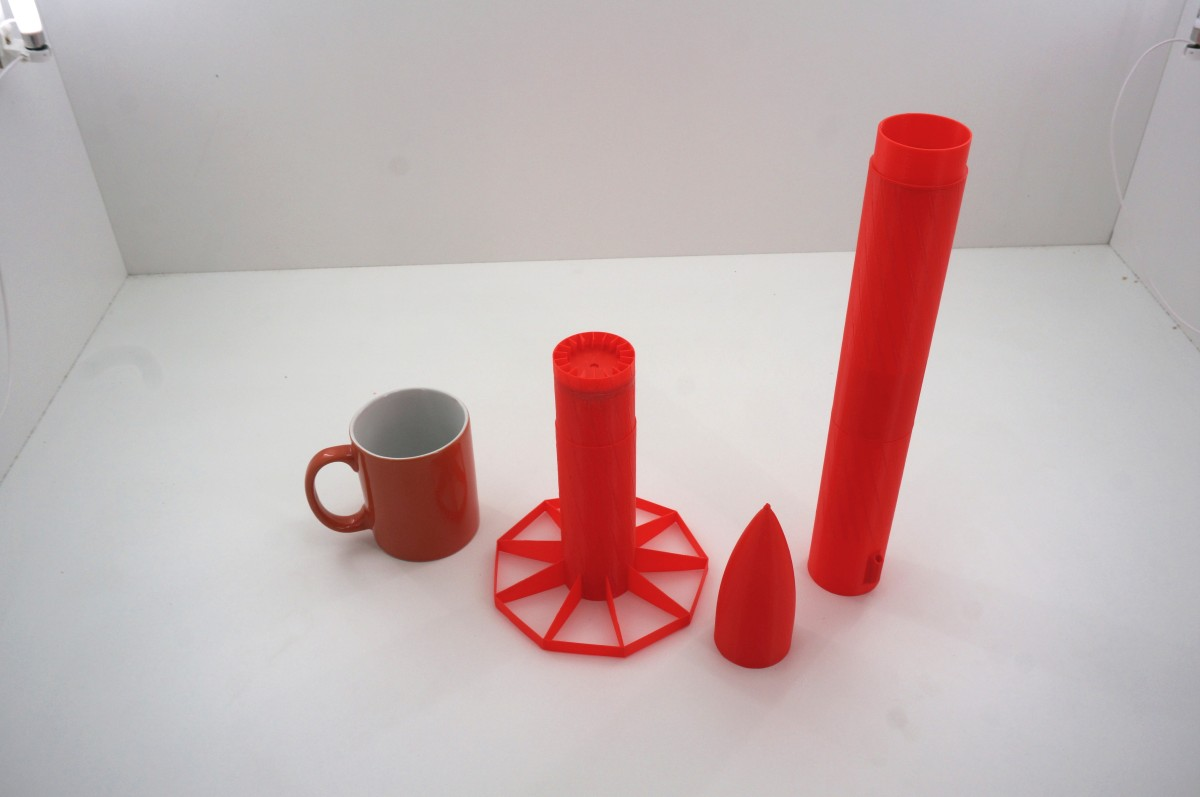
\includegraphics{./img/3dprinted_rocket_parts.jpg}}
\caption{A sample of printable rocket design. (Experimentally printed from red ABS)} 
\label{fig:printed_parts}
\end{center}
\end{figure}


\subsection{Rocket body and recovery system}

The rocket body is designed as simple as possible to minimize quality parameter demands posed on the used 3D printer. The following construction challenging details have been resolved until a current stage of rocket development. 

\begin{itemize}
\item Fins design
\item Rocket stage connections
\item Rocket hull reinforcements
\item Recovery system
\end{itemize}

The rocket body was designed in OpenSCAD modelling software. OpenSCAD is not an interactive modeller. Instead it is more like a 3D-compiler that reads script files that describe the object and renders the 3D model from these script files. This gives the 3D designer a full control over the modelling process and enables to easily change any step in the modelling process or to make designs that are defined by configurable parameters.
Specifically, the parametric modelling basis of OpenSCAD is used several times in the rocket design because it allows to make model shape and number of construction elements related to the size of the rocket.  One example involve spiral reinforcements in the rocket hull, where the number of ribs and their shape is dependent on rocket hull diameter and wall thickness. 

The rocket body was divided into tree parts. The engine stage, payload stage and recovery stage. Each of these parts are interconnected by specially designed interlock module. The design of stage connection must met several criteria. 

\begin{itemize}
\item Low mass
\item Robustness
\item Must withstand radial, torque and axial forces without considerable deformations
\item Repeatable coupling 
\item 3D Printability
\end{itemize}

Several classical construction solutions for that stage connection such as threaded connection, bung mating etc. were tested.
The final solution was the use of a circular embossment on both stages. The embossments fit into each other and due to the elasticity of hull material hold the connection surfaces in place.  The strength of interconnection could be adjusted to the rocket size by adjusting the number of embossments and their size.

Another unique construction solution on the rocket design are fins. The rocket fins are aero-dynamical stabilization surfaces needed for smooth stable ballistic trajectory flight.  The classical planar fins are very well known, but this type of fins is not suitable for printed model.  The long wingspan and elastic properties of PLA material tend to vibrate under high speed airflows.
Therefore, an alternative fins construction was considered - the so called grid-fins design \cite{grid_fins} where the elasticity of material is suppressed heavily by an orthogonal bonding.
Grid fins design expects the wall of grid material opposite to the grid cross-section to be very thin. This assumption significantly limits the range of printable rocket sizes. The limits arise from the fact that most 3D printers have 0.4 mm nozzle diameter. Therefore the extrusion width of that printer cannot be less than approximately 0.5 mm. Such grid-fin wall size cannot be used in rockets with fins' wingspan smaller than approximately 7 cm, because the aero-dynamical drag of such grid fin is too large. 

\begin{figure}[ht]
\begin{center}
\resizebox{\linewidth}{!}{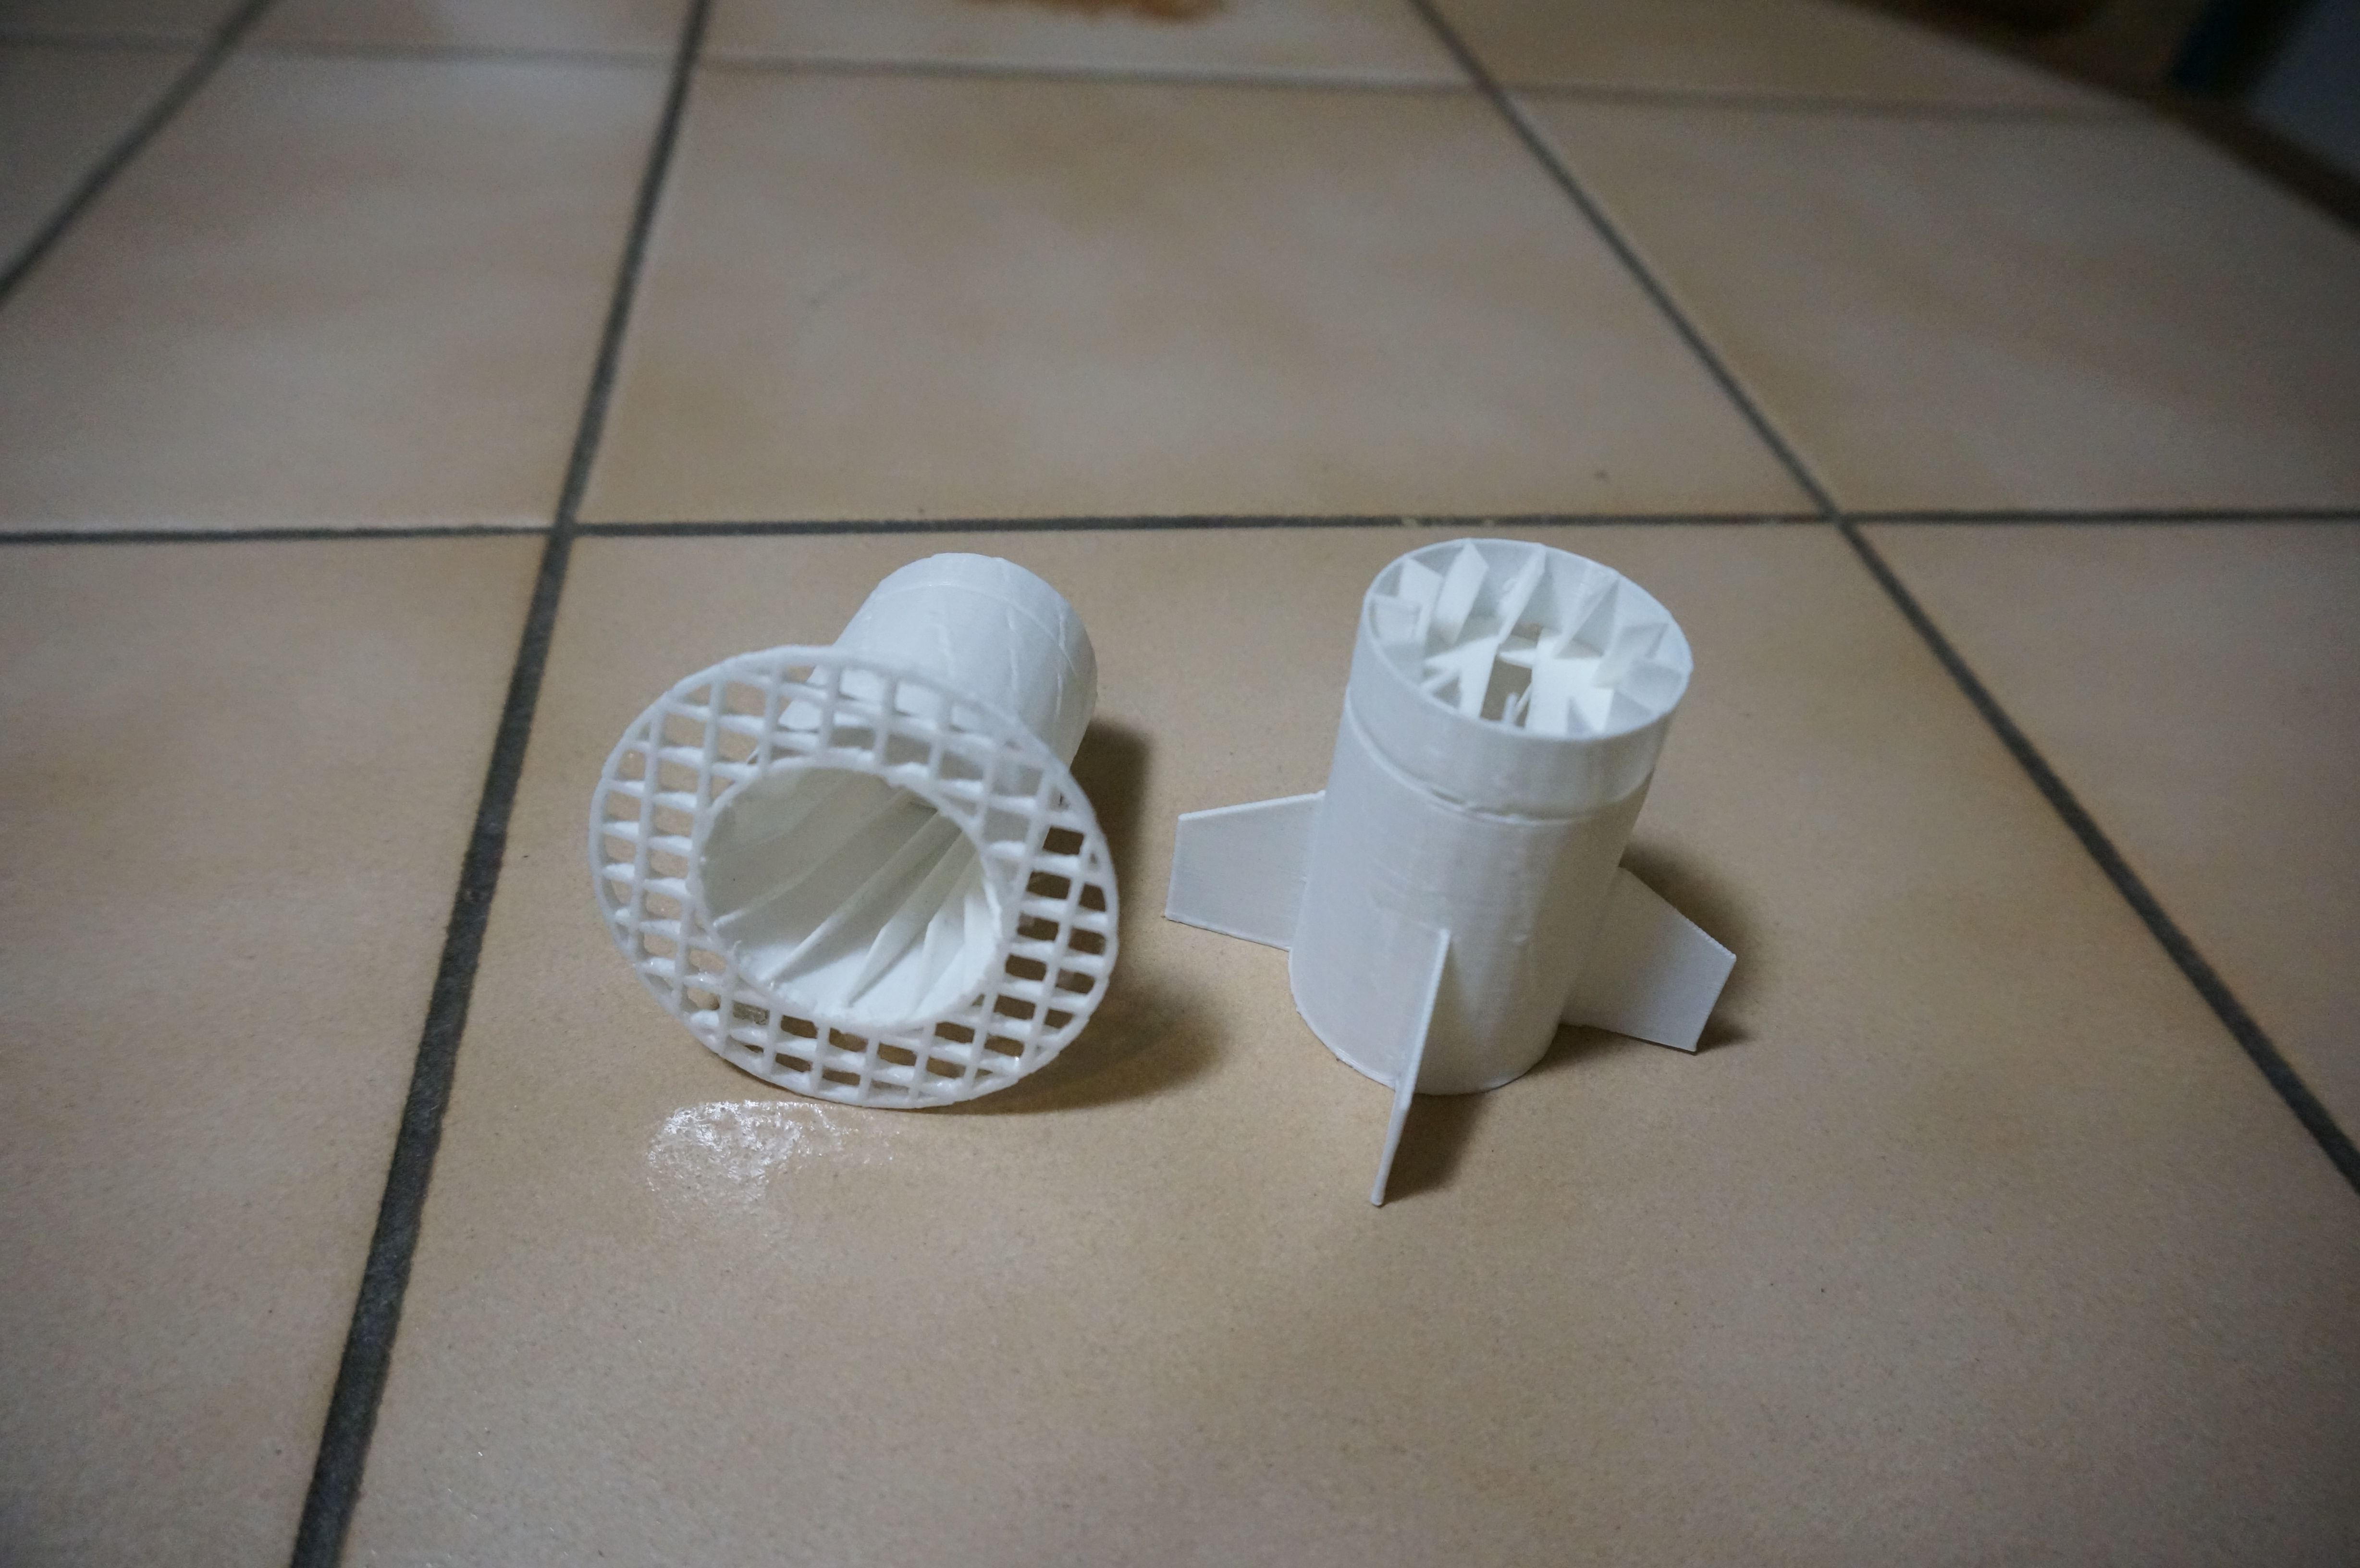
\includegraphics{./img/3d_printed_grid_fin.jpg}}
\caption{A reduced size model of grid fin based on the engine stage of the rocket. (Printed from PLA material) } 
\label{fig:grid_fin}
\end{center}
\end{figure}


The drag must be reduced to achieve usable ceiling parameters. To overcome this issue a hybrid grid-fins were developed as a compromise between rigidity of grid-fins and aerodynamic efficiency of classic planar fins. 


\subsection{3D printable rocket engine}

Several technical solutions were considered and tested during the rocket development. 

\begin{itemize}
\item Reusable metal case engine
\item Disposable model rocket engine
\item Experiment with one-off use of 3D printed engine
\end{itemize}

A reusable metal engine shown in figure \ref{fig:metal_engine} was used in the very first rocket design (which was not actually 3D printed). The testing rocket with reusable engine was lunched, but the recovery was unsuccessful. The parachute recovery system failed and rocket had to be excavated from soil in the test field. Consequently the reusable rocket engine was mechanically deformed and could not be used any more.
The reusable rocket engine was quite expensive and recovery system failure or some other system failure which cause engine lost could not be prevented completely in the future. Therefore the use of reusable rocket engine was evaluated as unsuitable for experimental rocket design. 
The commercial disposable model rocket engine was used in another small, but this time 3D printed rocket design. The rocket lunch was partiality successful because the 3D printed rocket withstood the stress forces during the launch.  But parachute recovery system failed again. 

\begin{figure}[ht]
\begin{center}
\resizebox{\linewidth}{!}{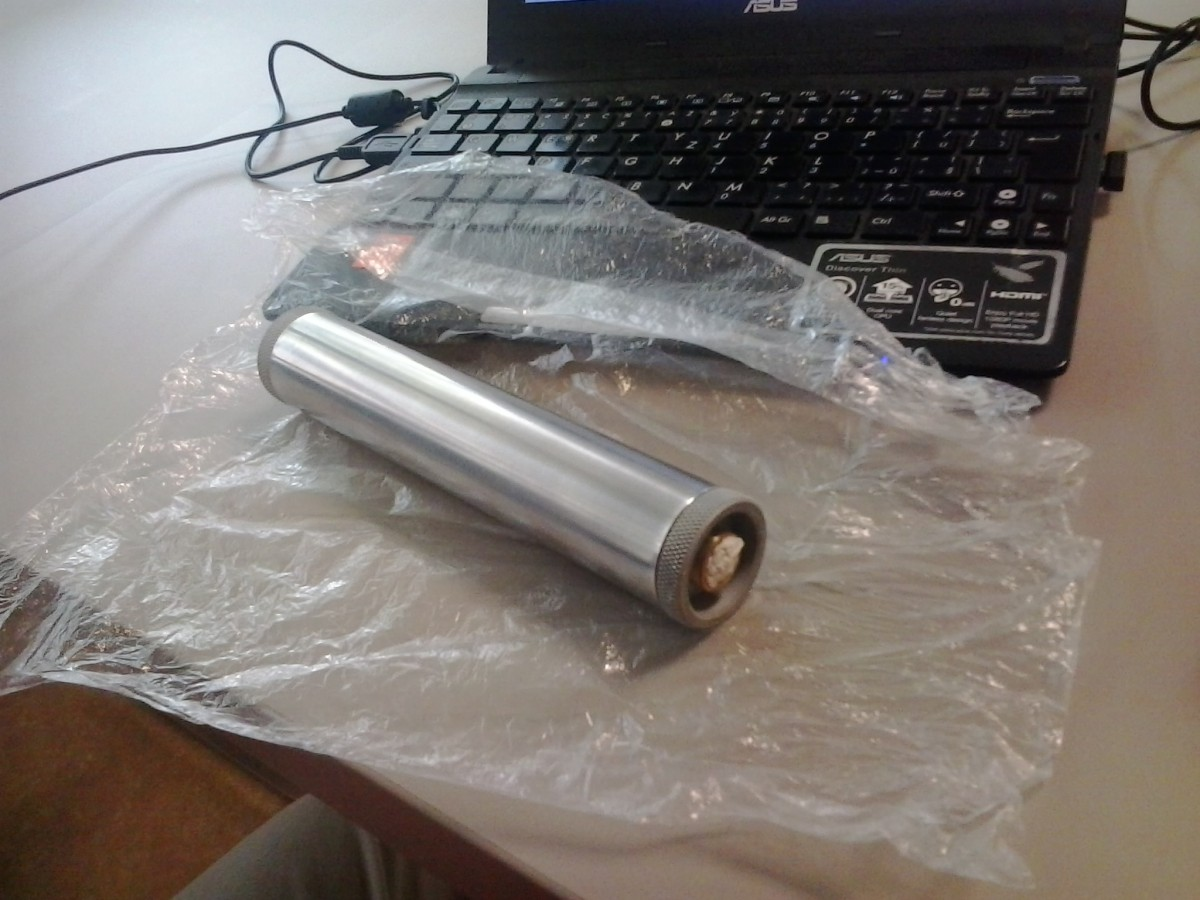
\includegraphics{./img/rocket_engine1.jpg}}
\caption{Reusable commercial rocket engine with specific impulse of 160 Ns} 
\label{fig:metal_engine}
\end{center}
\end{figure}

As result of this experiment the 3D printable rocket engine integrated directly to the engine stage was considered as the best option. The construction of plastic 3D printed solid fuel rocket engine is challenging task because the engine chassis must resist to high temperatures and pressures. Therefore first static test of printed engines expectedly failed, fortunately the extreme condition are active only for a short time (several seconds the most). As consequence of that a rocket engine could have self cooled lost material design which allows safe operation over whole thrust generating flight phase. 


\section{Conclusion}

A considerable amount of development work resulted in a partially usable 3D printable rocket model. The FDM technology was proven to be a right selection. But large amount of development work will be needed to finish the rocket design to the level which will allow an easy usage by students. 
Specifically the following problems must be resolved before widespread usage: 

\begin{itemize}
\item Reliable recovery system
\item Easily producible rocket engine design  
\item On board avionics which could universally provide power source, recovery and measurement functions for any student payload. 
\end{itemize}

\section*{Acknowledgements}

The research presented in this proposal was not supported from any grant or from public resources. It was funded exclusively by participants of Summer Astronomical School in Upice and by Universal Scientific Technologies s.r.o. 

%----------------------------------------------------------
%               THIS IS THE PLACE FOR REFERENCES
\begin{thebibliography}{9}
\bibitem{rocket_sounding}
NASA Sounding Rockets User Handbook, Sounding Rockets Program Office,Sub-orbital and Special Orbital Projects Directorate
NASA Goddard Space Flight Center,Wallops Flight Facility, 23.3.2016 [online] http://sites.wff.nasa.gov/code810/files/SRHB.pdf
\bibitem{grid_fins}
Zaloga, Steve (2000). The Scud and Other Russian Ballistic Missile Vehicles. New Territories, Hong Kong: Concord Publications Co. ISBN 962-361-675-9.
\bibitem{openscad}
Marius Kintel et al.  23.3.2016 [Online]
http://www.openscad.org/about.html
\end{thebibliography}


%----------------------------------------------------------
%               THIS IS THE PLACE FOR AUTHOR CV
\begin{authorcv}{Jakub Kakona}
He is a Ph.D. student of  Air Traffic Control programme under Electrical Engineering and Information Technology. His professional activities are radioastronomy, development of 3D printers and scientific instruments design. 
\end{authorcv}
\end{document}

